% Copyright (c)  2019  FSC.
% Permission is granted to copy, distribute and/or modify this document
% under the terms of the GNU Free Documentation License, Version 1.3
% or any later version published by the Free Software Foundation;
% with no Invariant Sections, no Front-Cover Texts, and no Back-Cover Texts.
% A copy of the license is included in the section entitled "GNU
% Free Documentation License".

\chapter{Visual Design}\label{chap:visual-design}
Nella terza fase, le attività che sono state svolte riguardano:
\begin{itemize}
	\item La progettazione dei layout grafici
	\item Costruzione dei template HTML
	\item Costruzione del prototipo di comunicazione
\end{itemize}
L'obiettivo è quello di definire in dettaglio la grafica del sito attraverso la 
realizzazione dei layout grafici (cioè, andare a completare il prototito di navigazione).

Si disegnano menù, intestazioni e decorazioni, si scelgono i colori, lo stile dei 
caratteri, le immagini da utilizzare. Infatti, come team, si è deciso di utilizzare 
queste specifiche:
\begin{itemize}
	\item Le dimensioni delle immagini e delle icone sono adattate alla pagina, in base 
	alla risulozione dello schermo sul quale si sta visionando la pagina web.
	\item Dal punto di vista estetico, si è fatto uso di diverse sfumature di colore per 
	dare la possibilità di riconoscere intuitivamente l'area su cui si sta navigando, 
	seguendo le linee guida del Material Design:
	\begin{itemize}
		\item Elevazioni:
		\begin{itemize}
			\item Elevazione 0dp: \textbf{\#121212} 
			\item Elevazione 1dp: \textbf{\#1e1e1e}
			\item Elevazione 2dp: \textbf{\#232323}
			\item Elevazione 3dp: \textbf{\#252525}
			\item Elevazione 4dp: \textbf{\#272727}
			\item Elevazione 6dp: \textbf{\#2c2c2c}
			\item Elevazione 8dp: \textbf{\#2e2e2e}
			\item Elevazione 12dp: \textbf{\#333333}
			\item Elevazione 16dp: \textbf{\#363636}
			\item Elevazione 24dp: \textbf{\#383838}
		\end{itemize} 
		\item Colore primario: \textbf{\#FF9800}
		\item Colore secondario: \textbf{\#6c757d}
		\item Font: \textbf{Raleway} 
	\end{itemize}
\end{itemize}
Di seguito sono riportati i colori utilizzati su AdobeXD per creare i prototipi di 
navigazione riportati di seguito.

\begin{figure}
	\centering
	\begin{minipage}[c]{0.45\textwidth}
		\centering
		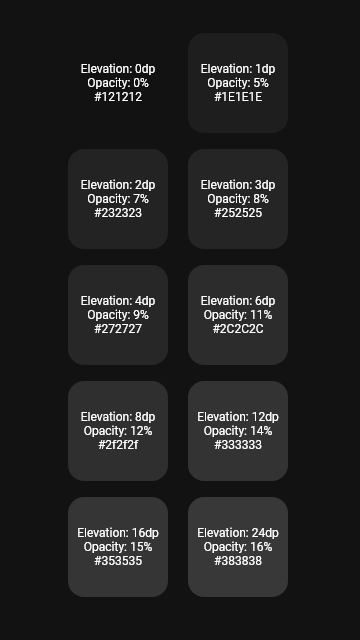
\includegraphics[width=3.0in]{images/prototipo-comunicazione/Colors-Black}
		\caption{Colori di elevazione}
		\label{fig:colori:elevazioni}
	\end{minipage}~\begin{minipage}[c]{0.45\textwidth}
		\centering
		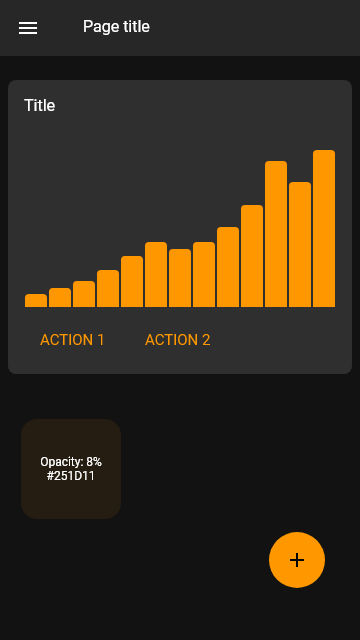
\includegraphics[width=3.0in]{images/prototipo-comunicazione/Colors-Primary}
		\caption{Colori primari}
		\label{fig:colori:primari}
	\end{minipage}
\end{figure}

\section{Layout grafici}\label{sec:layout-grafici}
Per visionare i layout grafici del sistema si è scelto di riportare di seguito 
i prototipi di comunicazione realizzati con AdobeXD.

% Copyright (c)  2019  FSC.
% Permission is granted to copy, distribute and/or modify this document
% under the terms of the GNU Free Documentation License, Version 1.3
% or any later version published by the Free Software Foundation;
% with no Invariant Sections, no Front-Cover Texts, and no Back-Cover Texts.
% A copy of the license is included in the section entitled "GNU
% Free Documentation License".

\begin{figure}[H]
	\centering
	\caption{Prototipo di comunicazione: pagina di login (1).}
	\label{fig:prototipo-comunicazione:login-1}
	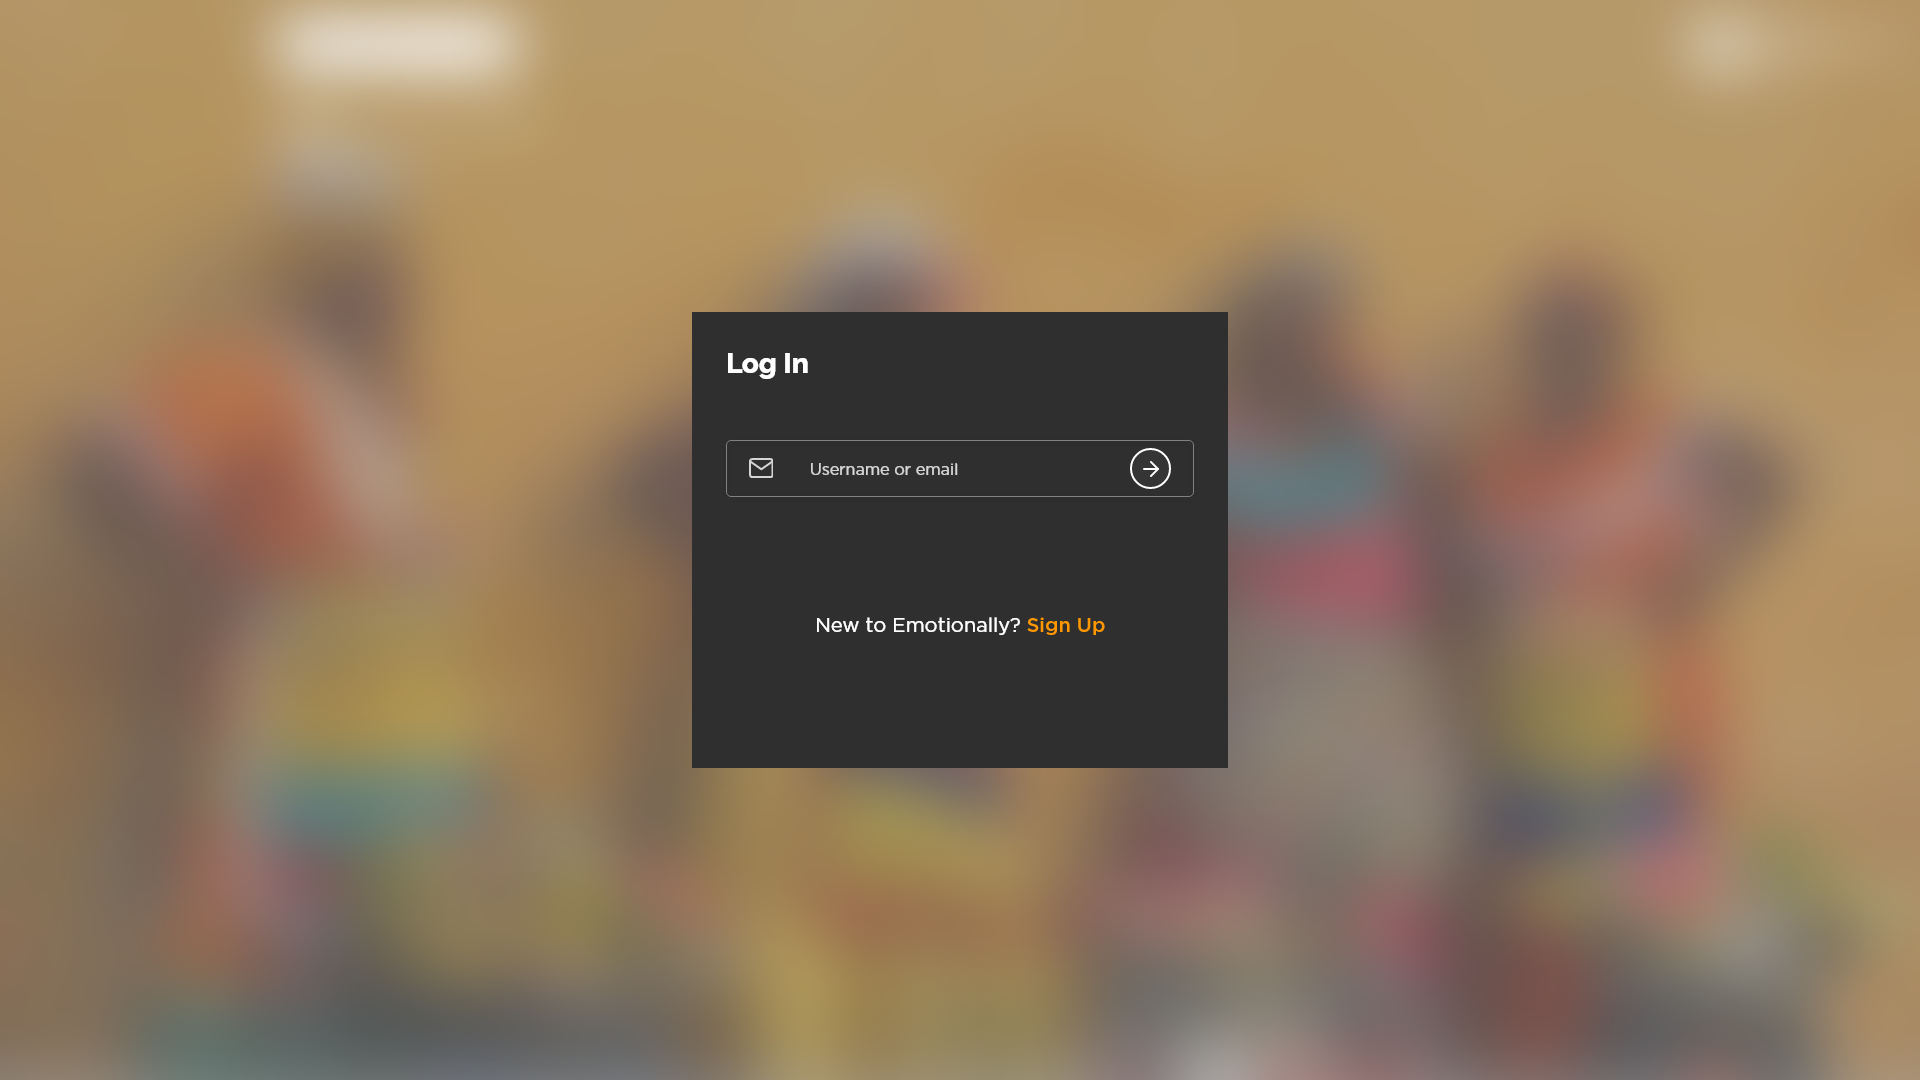
\includegraphics[width=\textwidth]{images/prototipo-comunicazione/login-1.png}
\end{figure}

\begin{figure}[H]
	\centering
	\caption{Prototipo di comunicazione: landing page.}
	\label{fig:prototipo-comunicazione:landing-page}
	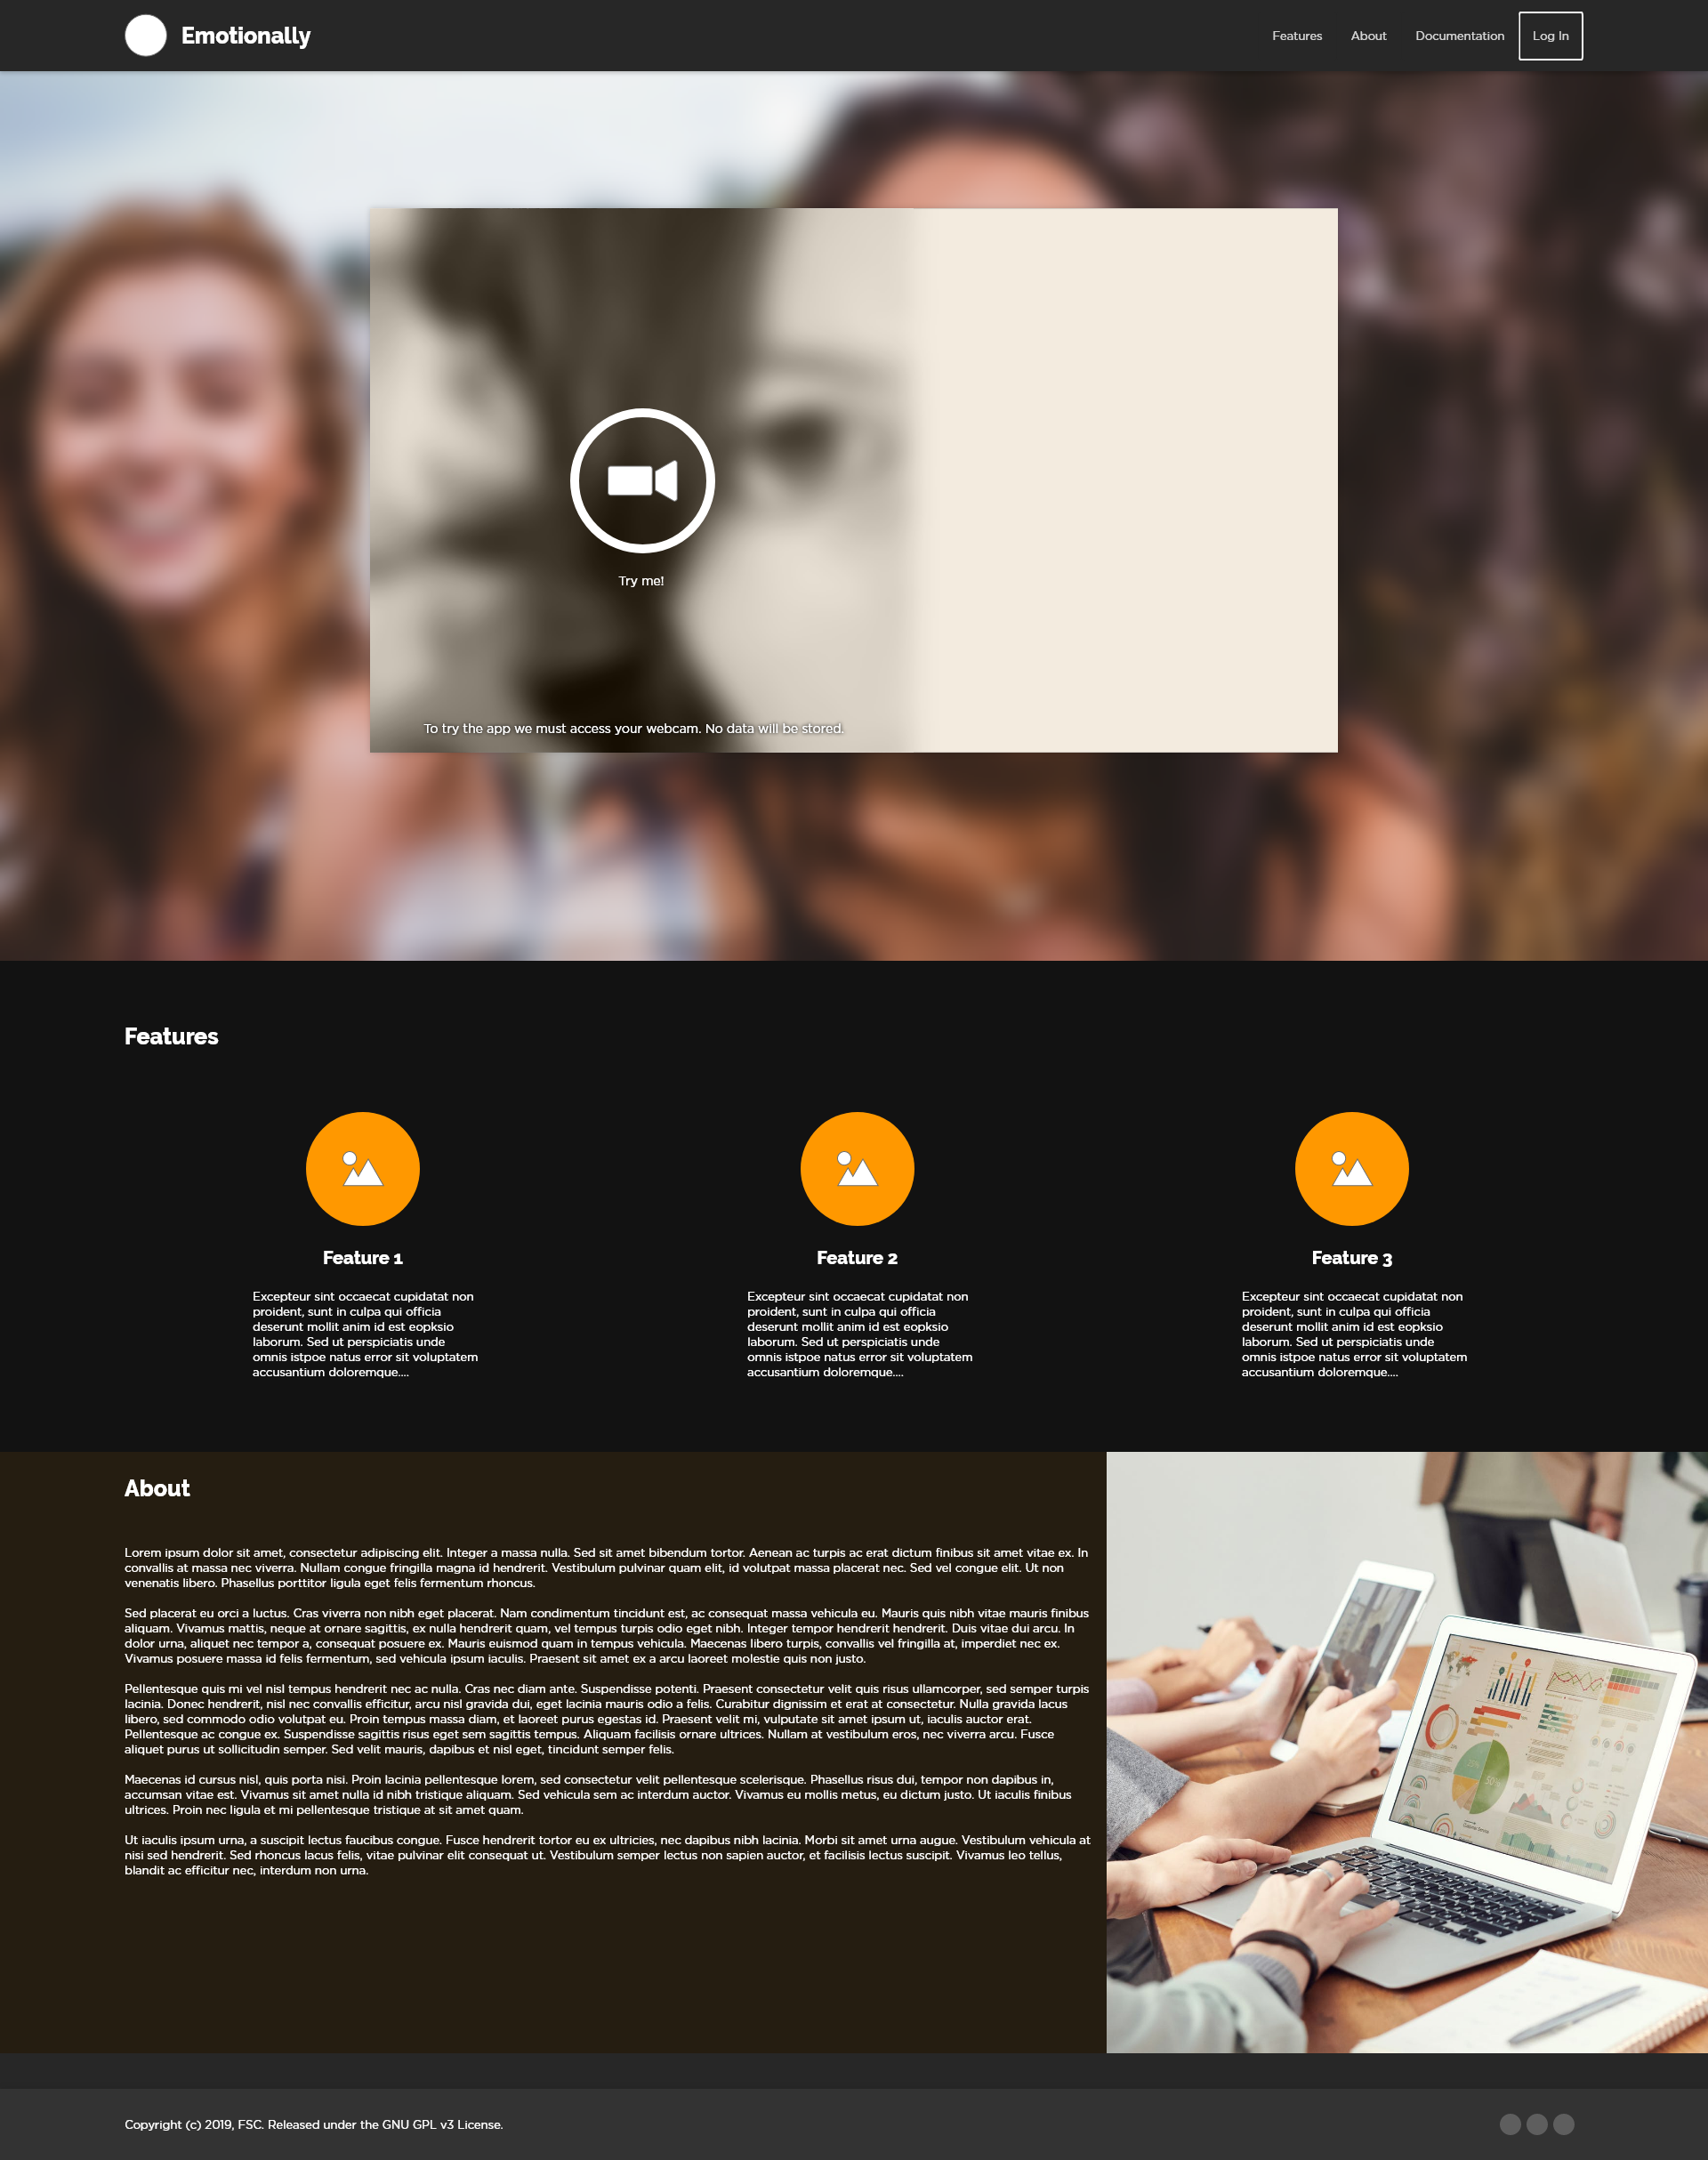
\includegraphics[width=\textwidth]{images/prototipo-comunicazione/Landing.png}
\end{figure}

\begin{figure}[H]
	\centering
	\caption{Prototipo di comunicazione: pagina di login (2).}
	\label{fig:prototipo-comunicazione:login-2}
	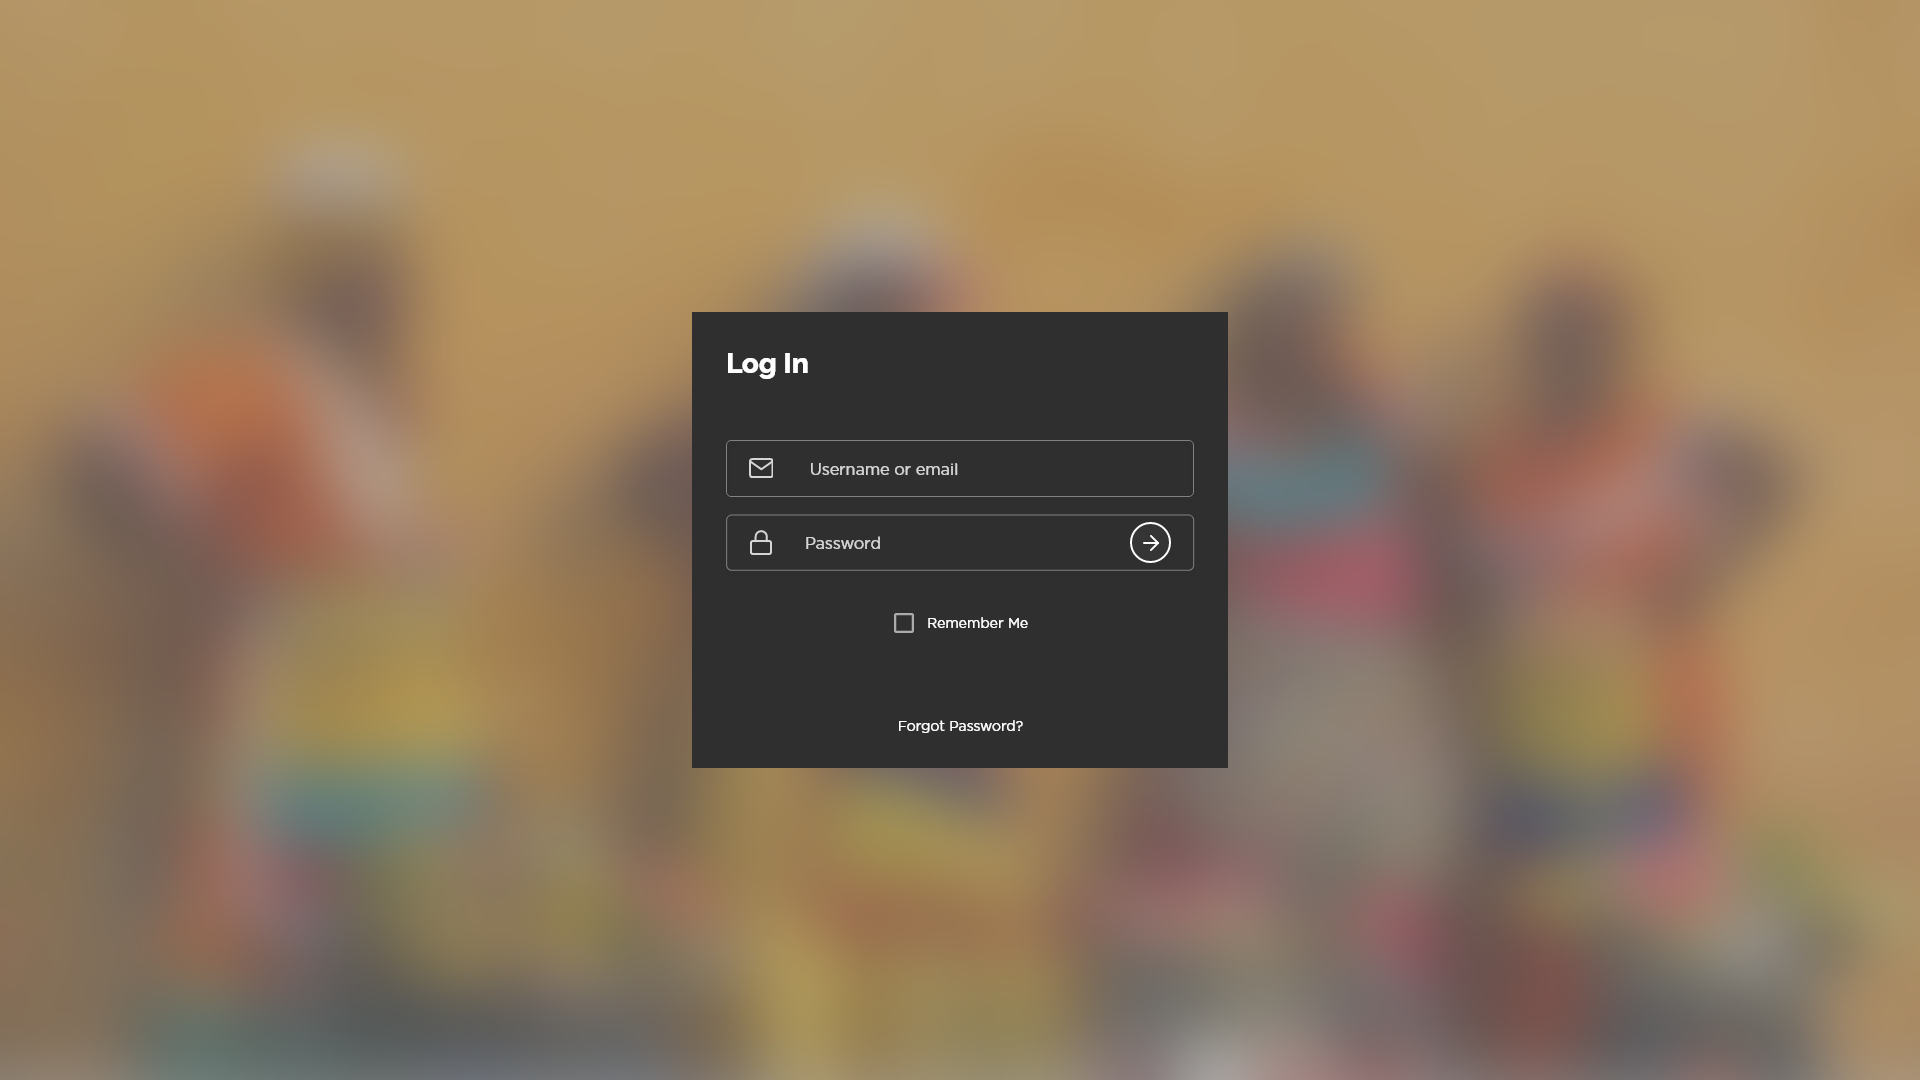
\includegraphics[width=\textwidth]{images/prototipo-comunicazione/login-2.png}
\end{figure}

\begin{figure}[H]
	\centering
	\caption{Prototipo di comunicazione: pagina di registrazione.}
	\label{fig:prototipo-comunicazione:registrazione}
	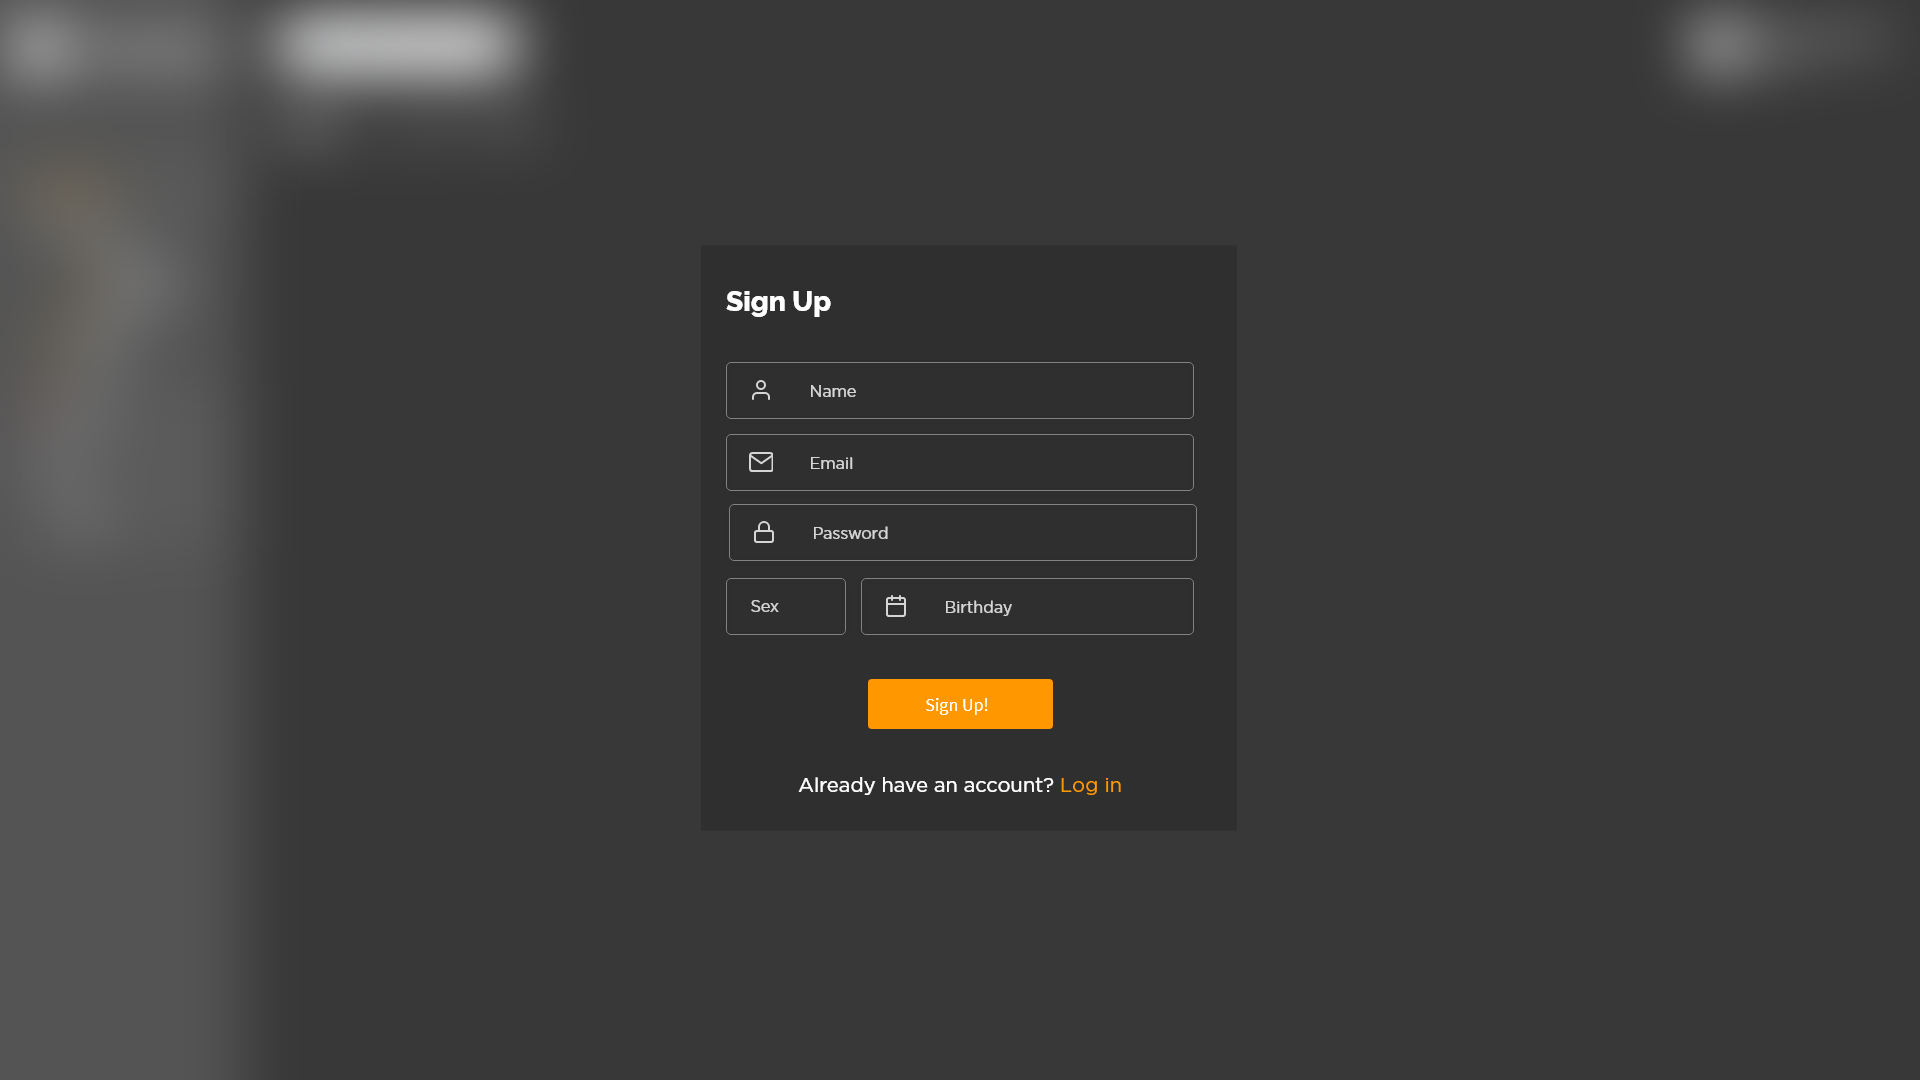
\includegraphics[width=\textwidth]{images/prototipo-comunicazione/registrazione.png}
\end{figure}

\begin{figure}[H]
	\centering
	\caption{Prototipo di comunicazione: pagina home.}
	\label{fig:prototipo-comunicazione:home}
	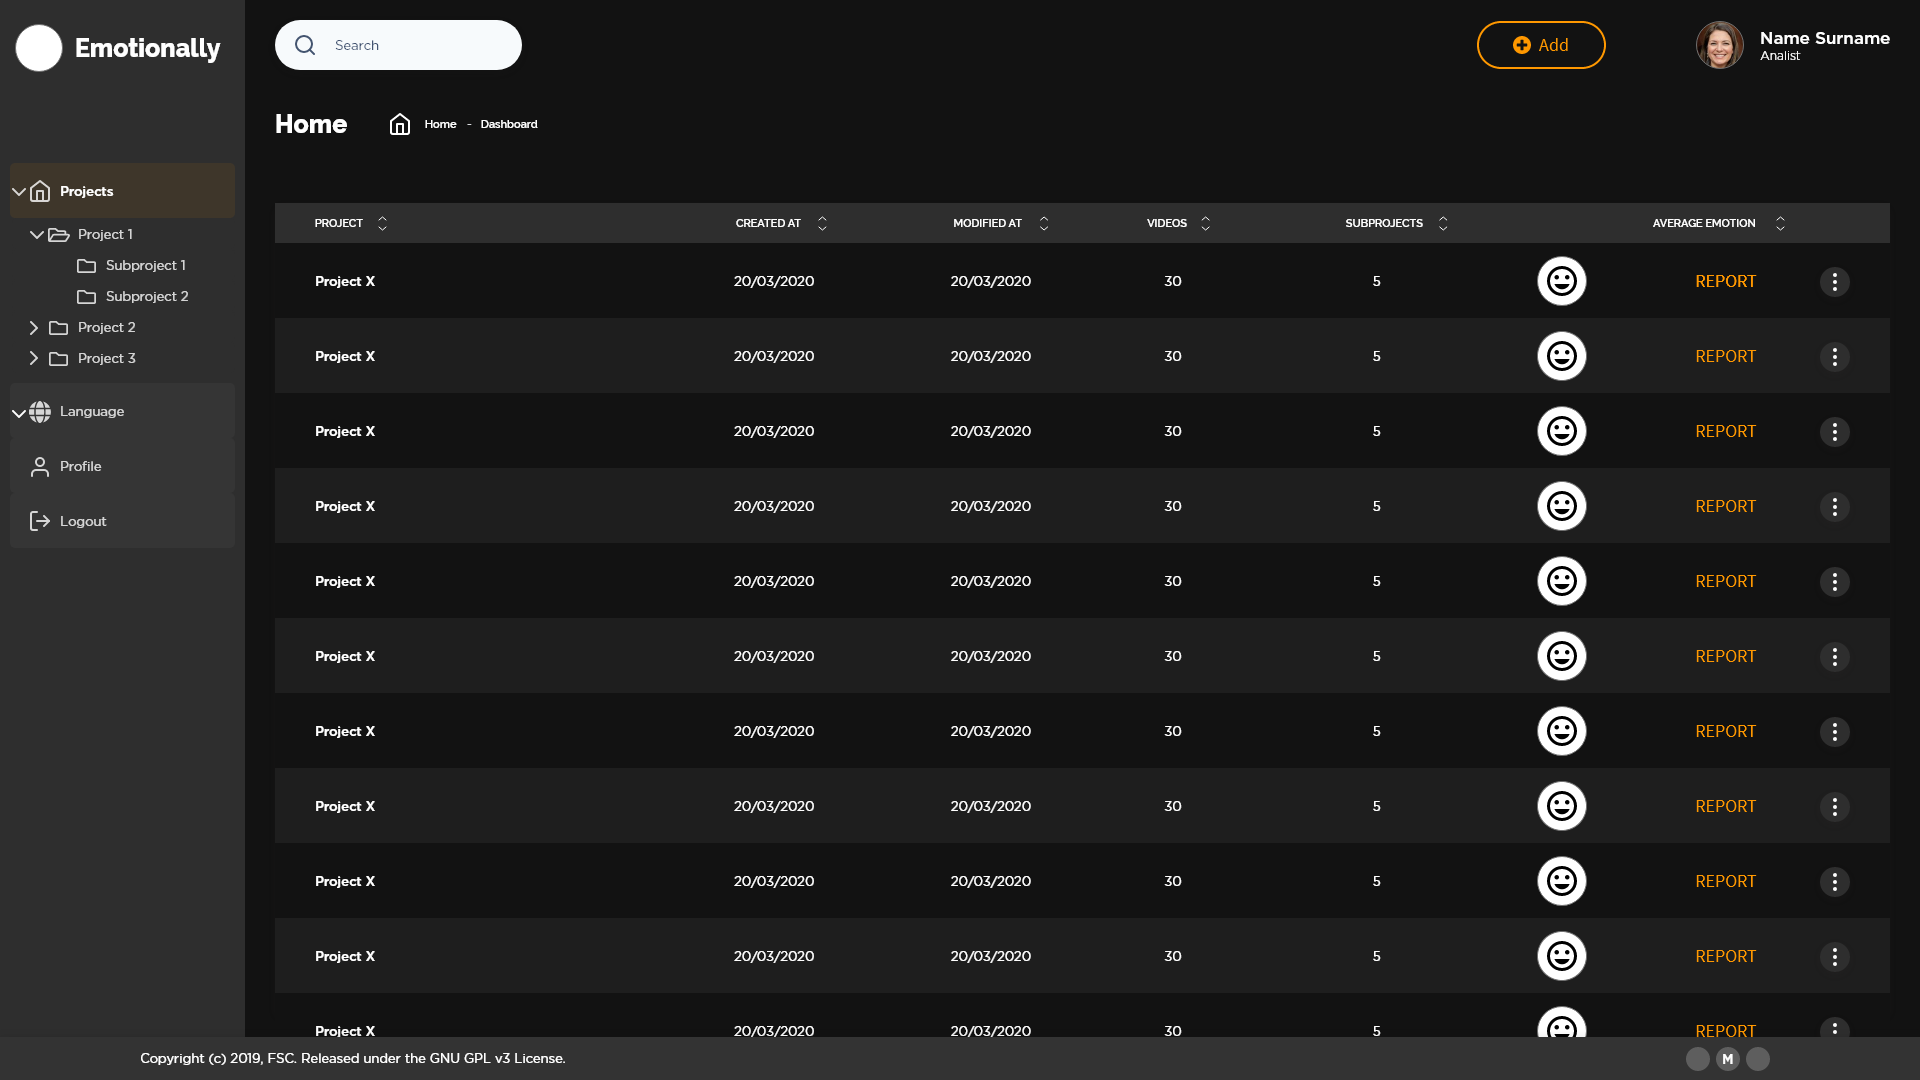
\includegraphics[width=\textwidth]{images/prototipo-comunicazione/home-no-scroll.png}
\end{figure}

\begin{figure}[H]
	\centering
	\caption{Prototipo di comunicazione: pagina di un progetto.}
	\label{fig:prototipo-comunicazione:project}
	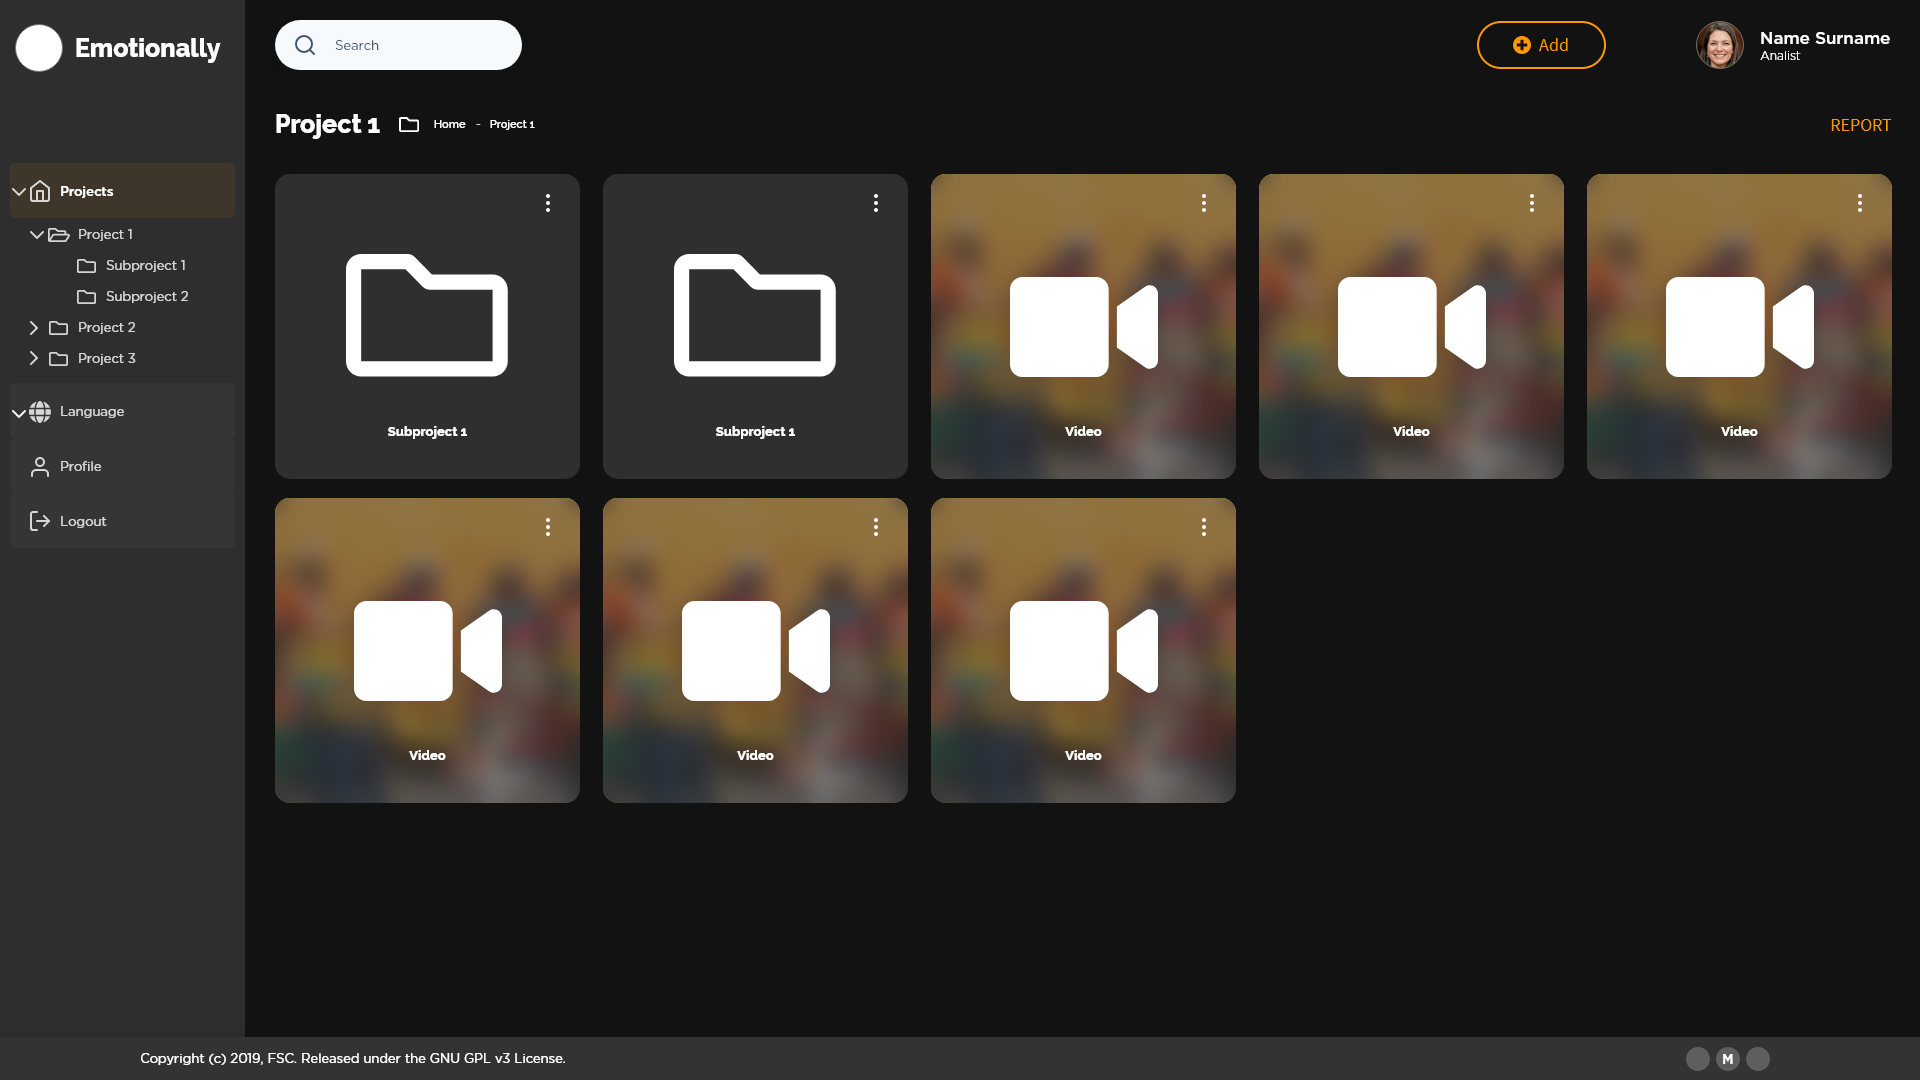
\includegraphics[width=\textwidth]{images/prototipo-comunicazione/project.png}
\end{figure}

\begin{figure}[H]
	\centering
	\caption{Prototipo di comunicazione: pagina di un sottoprogetto.}
	\label{fig:prototipo-comunicazione:subproject}
	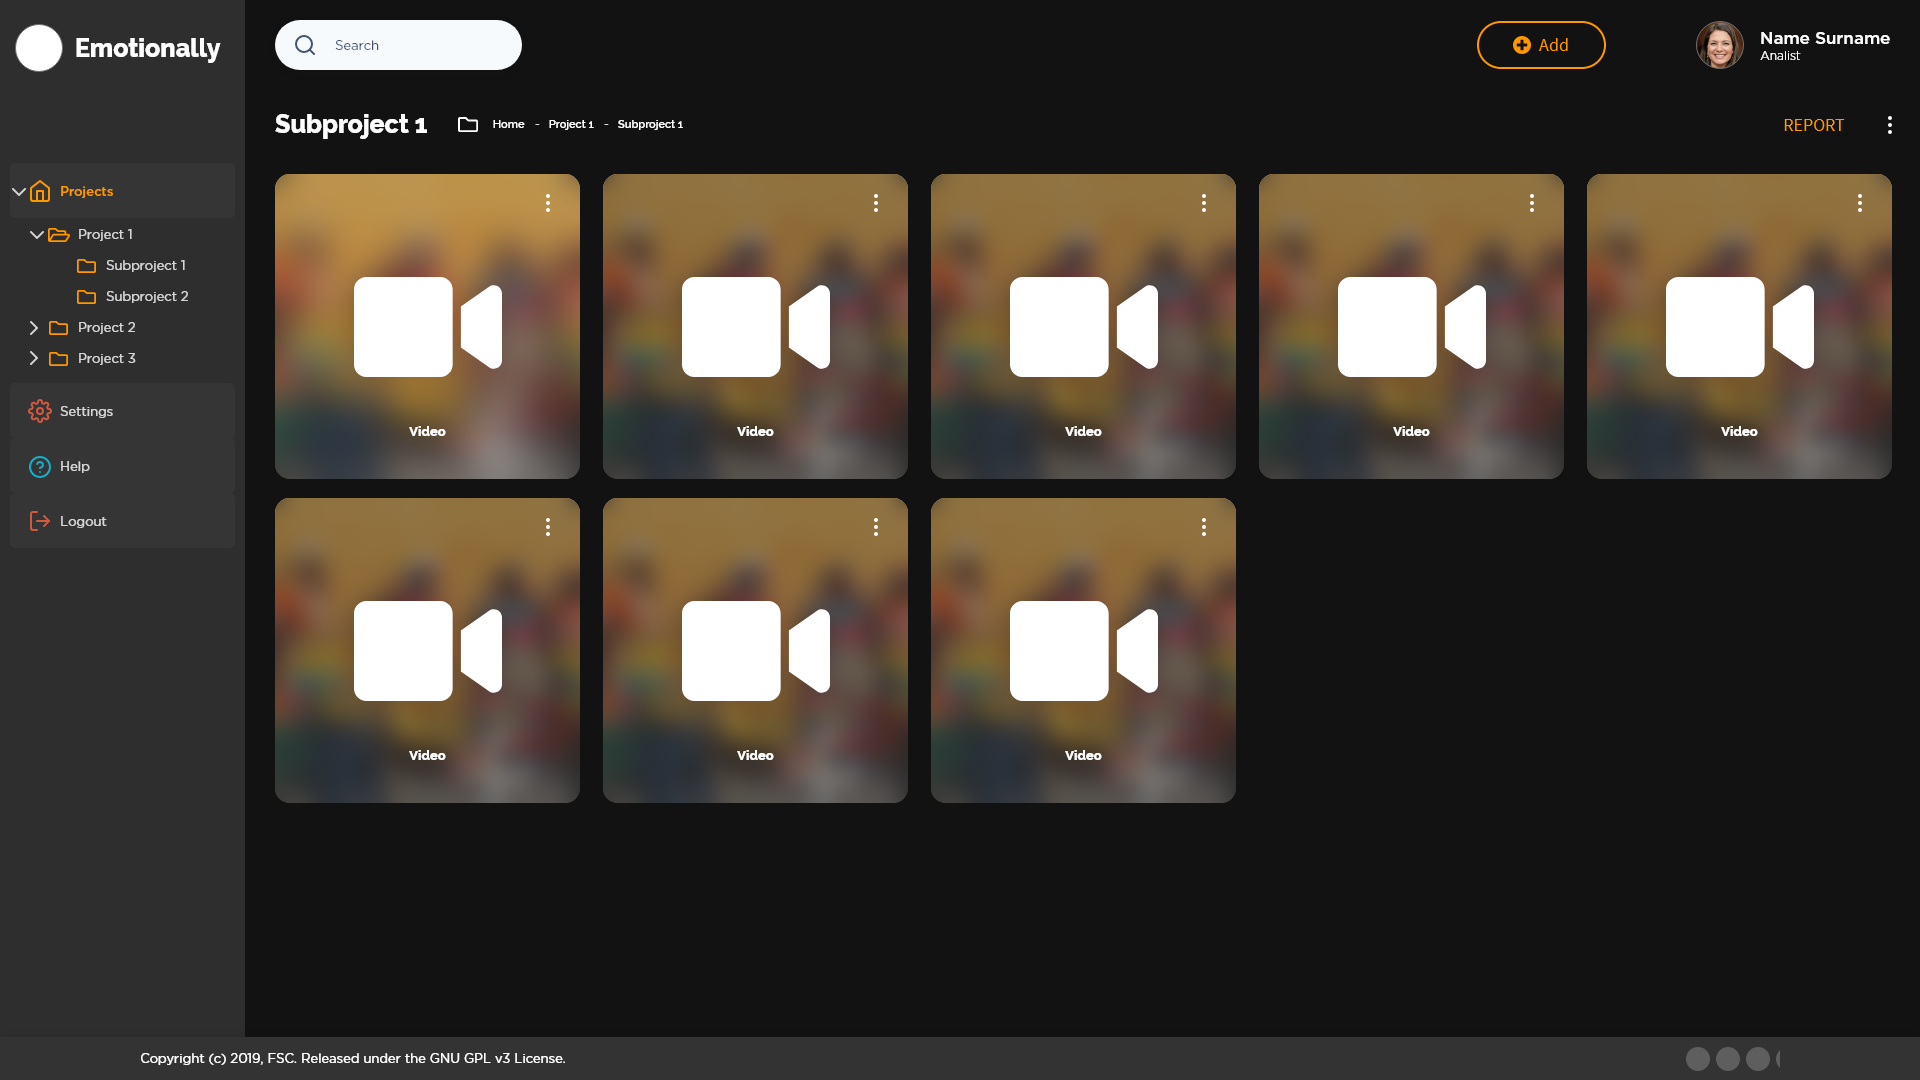
\includegraphics[width=\textwidth]{images/prototipo-comunicazione/subproject.png}
\end{figure}

\begin{figure}[H]
	\centering
	\caption{Prototipo di comunicazione: pagina di report di un video.}
	\label{fig:prototipo-comunicazione:video-report}
	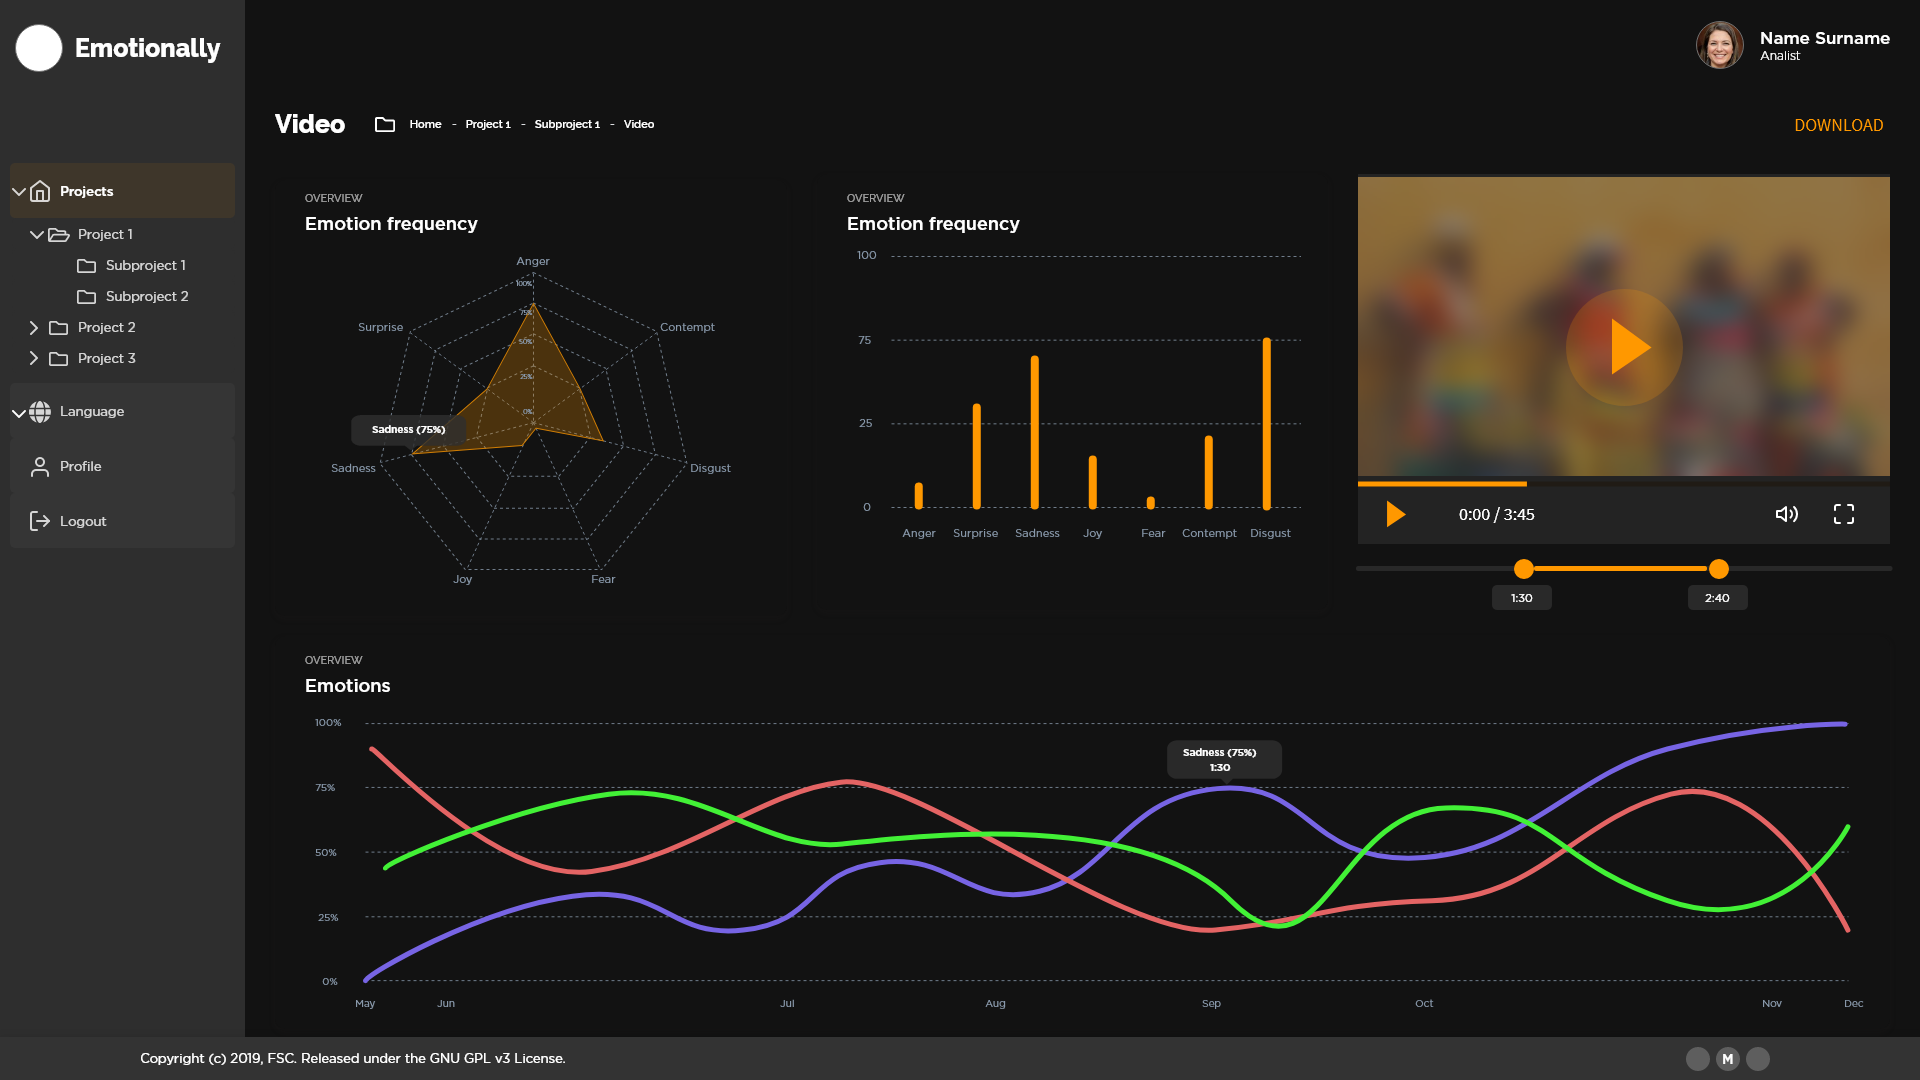
\includegraphics[width=\textwidth]{images/prototipo-comunicazione/report-video.png}
\end{figure}

\begin{figure}[H]
	\centering
	\caption{Prototipo di comunicazione: pagina di report di un progetto/sottoprogetto.}
	\label{fig:prototipo-comunicazione:project-report}
	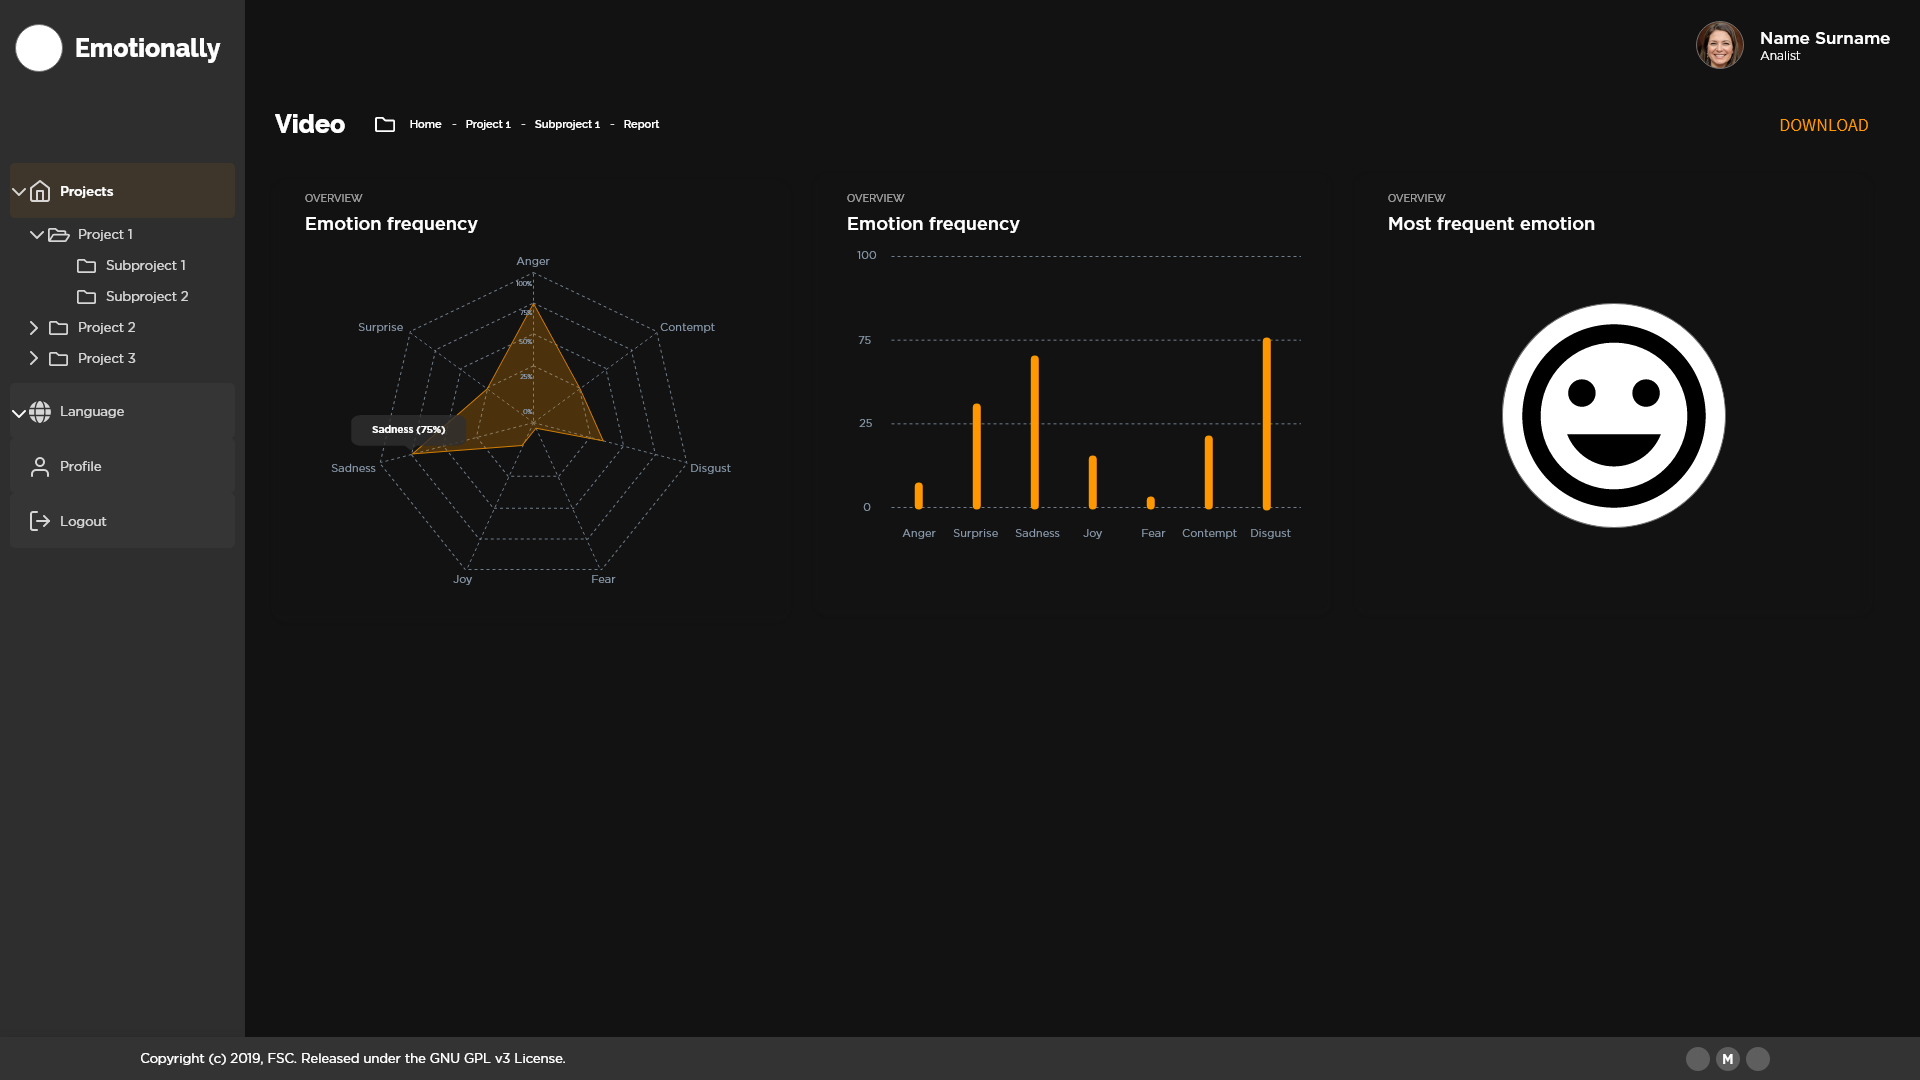
\includegraphics[width=\textwidth]{images/prototipo-comunicazione/report-project.png}
\end{figure}
